
\chapter{Stitching}

Für jeden Einspannzustand eines Bauteils können mehrere Bilddateien vorliegen.
Alle Bilddateien gehören zu dem gleichen Bauteil und müssen 
zusammengefügt werden, um ein einzelnes digitales Objekt zu erhalten. 
Als Voraussetzung ist gegeben das alle Bilder Überlappung enthalten.

Diese Überlappung kann benutzt werden, um die Bilder zu einem Objekt zusammenzufügen.
Das Zusammenfügen ist im folgenden auch Stitching genannt.
Für das Stitching von Bilddateien existieren schon mehrere Verfahren die in Bibliotheken
für viele Programmiersprachen implementiert sind. Der schon beschriebene ICP-Algorithmus
ist eines dieser Verfahren. Das Problem mit diesen Verfahren ist das sich zwei 
Datensätze angenähert werden indem auf ein Datensatz so lange eine 
Transformation und Rotation, manchmal auch eine Skalierung, angewendet wird, bis
die Distanz der Datensätze unter einen Grenzwert fällt oder nicht mehr verbessert
werden kann. Die Überlappung in den von dem Laserscanner aufgenommen Daten ist jedoch 
nur in zwei Achsen verschoben. Durch eine Rotation der Daten wird eine nicht korrekte 
Distanz berechnet.
Um die korrekte Transformation zu finden, mit der die beiden Bilder überlappen
muss nicht der komplette Bereich analysiert werden, sondern nur der überlappende Teil.
In diesem Bereich müssen Features erkannt werden. 
Nachdem in beiden Teilbildern Features erkannt wurden können diese miteinander
verglichen werden.

\section{Feature Erkennung}

Features in einem Bild sind große Unterschiede in benachbarten Pixeln. Die größten
Features sind die Ränder des Bauteils, kleinere Features können Oberflächenänderungen 
oder Spuren des Herstellungsprozesses sein. Diese Unterschiede können mithilfe 
der 'OpenCV' Bibliothek extrahiert werden. Diese Bibliothek gibt die erkannten 
Features als Liste von Konturen aus. Konturen selbst bestehen aus Listen von 
Punkten, die aus X und Y Koordinaten bestehen. Die Konturerkennung kann verbessert 
werden, indem das Bild entsprechend präpariert wird. In Abbildung \ref{fig:cons} und
\ref{fig:image_top} ist ein Ursprungsbild und die extrahierten Konturen zu sehen.
Mittig am linken und rechten Rand sind in Abbildung \ref{fig:image_top} 
Messfehler des Laserscanners zu sehen. Diese werden auch als Features in 
Abbildung \ref{fig:cons} erkannt. Diese müssen entfernt werden damit die Bilder 
korrekt zusammengefügt werden können. Erfolgt dies nicht werden diese Fehler miteinander
verglichen was das Ergebnis verfälscht.

\begin{figure}[h]
    \centering
    \includegraphics[width=0.8\textwidth]{images/with_con.jpg} % first figure itself
    \caption{Oberes Bild eines Scanvorgangs, FDM Bauteil}
    \label{fig:image_top}
\end{figure}

\begin{figure}[h]
    \centering
    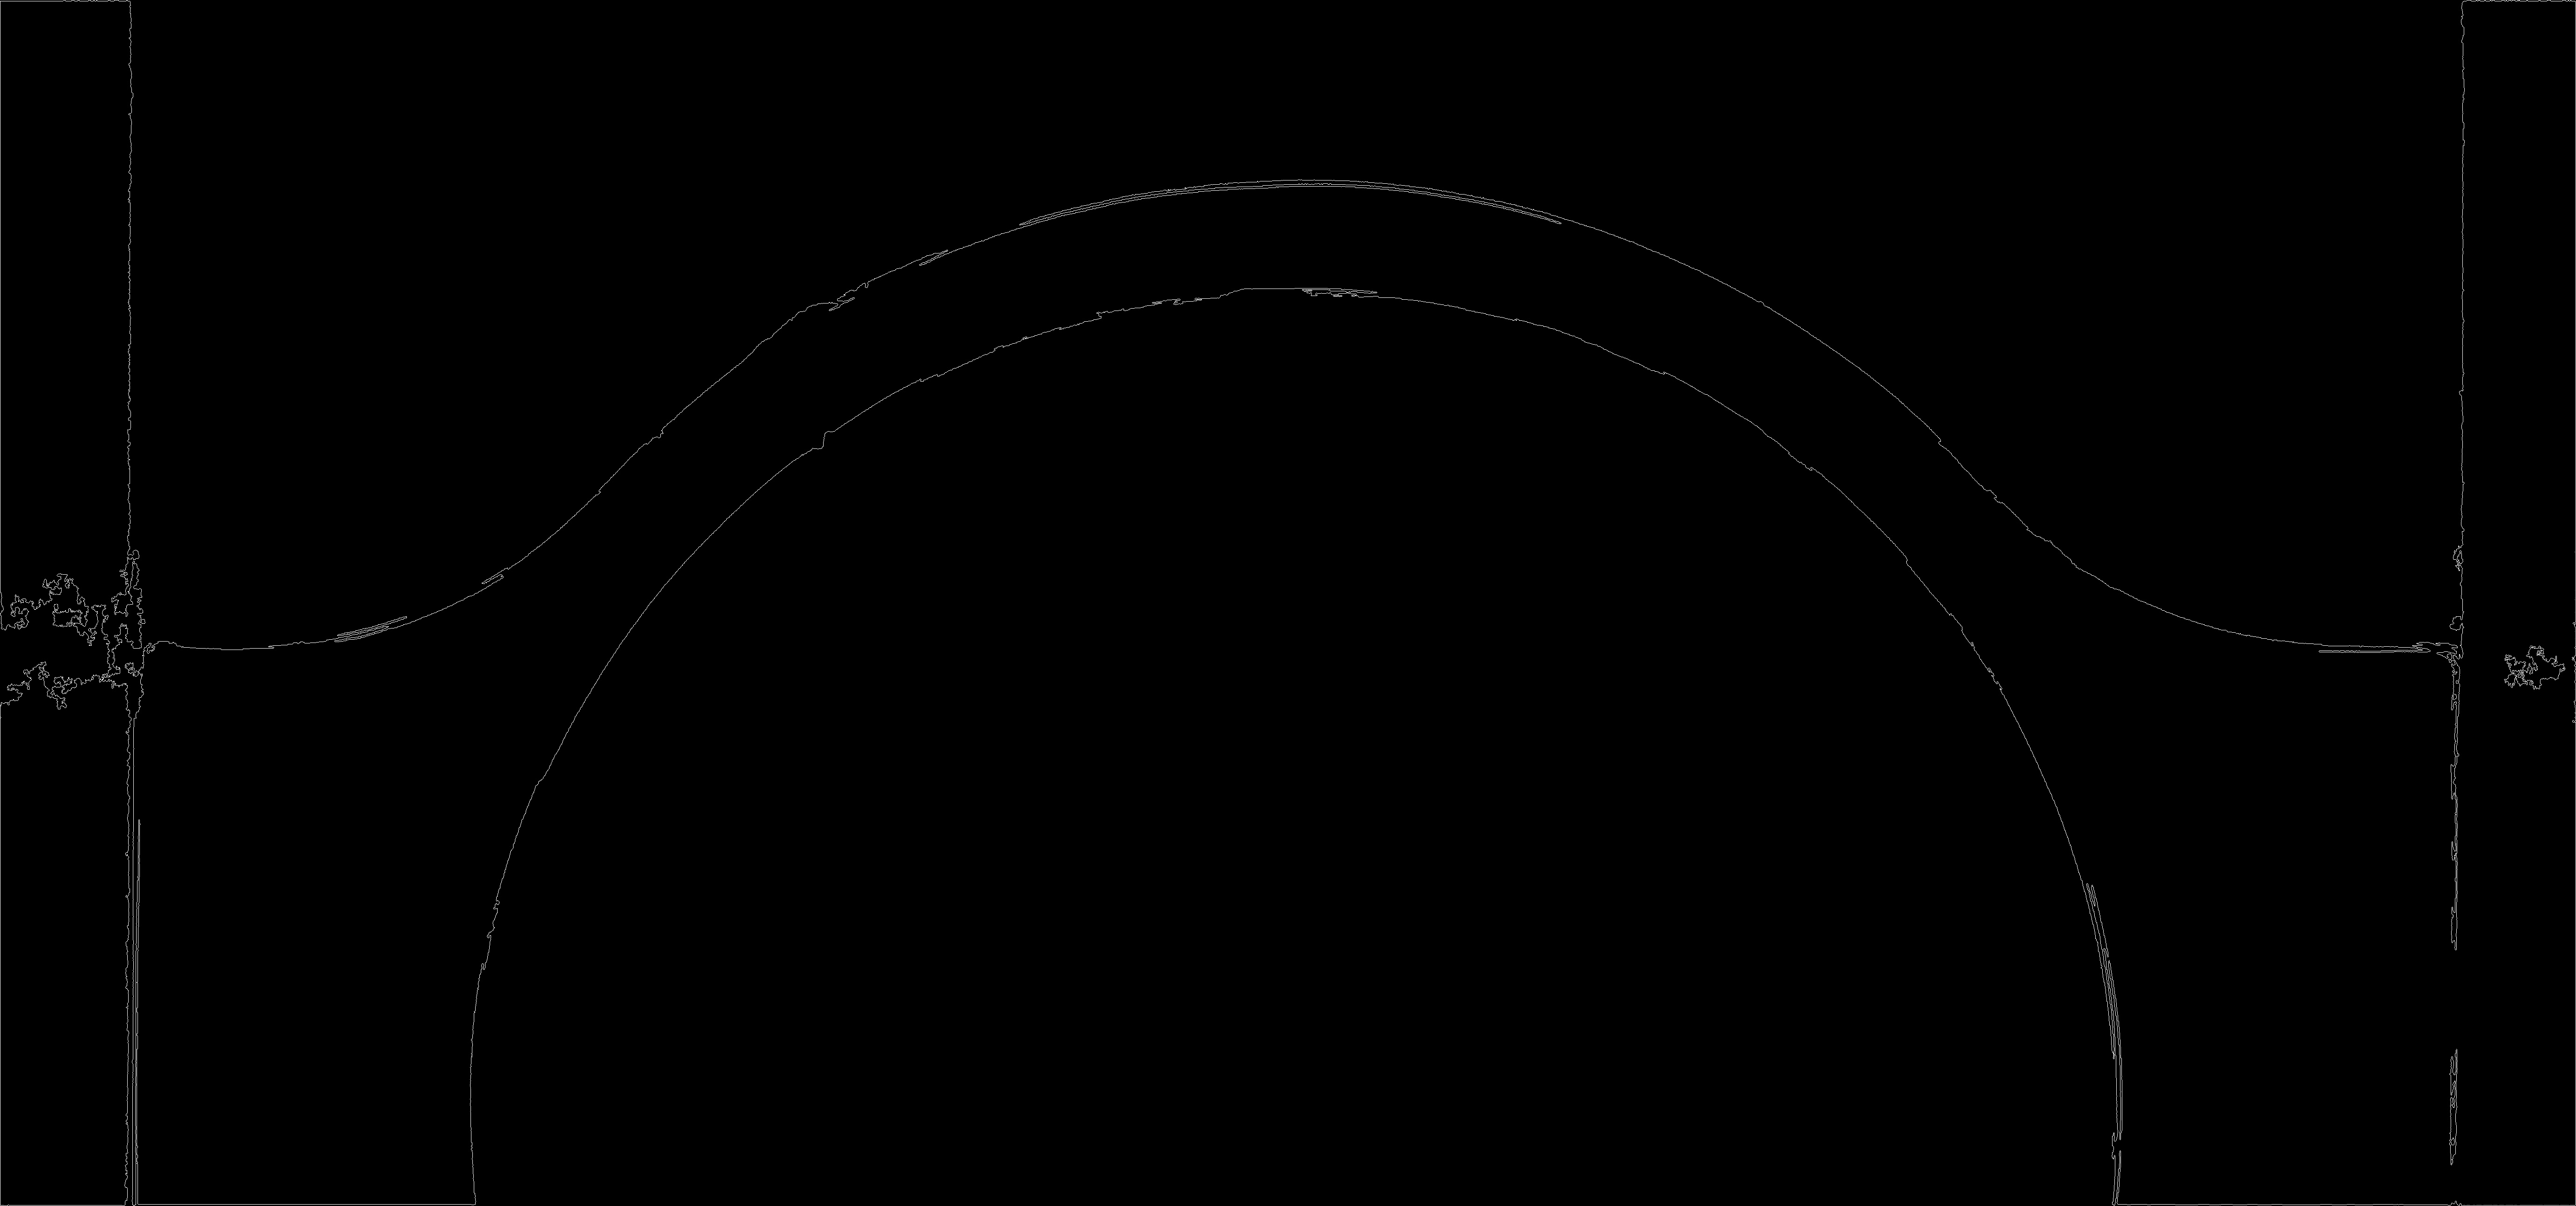
\includegraphics[width=0.8\textwidth]{images/only_con.jpg} % second figure itself
    \caption{Extrahierte Kontouren des Bildes ohne Pre-Processing}
    \label{fig:cons}
\end{figure}

Die Überlappung kann nur im oberen oder unteren Bildbereich auftreten. Der restliche 
Teil des Bildes kann also entfernt werden. So wird außerdem Rechenzeit gespart.

\begin{figure}[h]
    \centering
    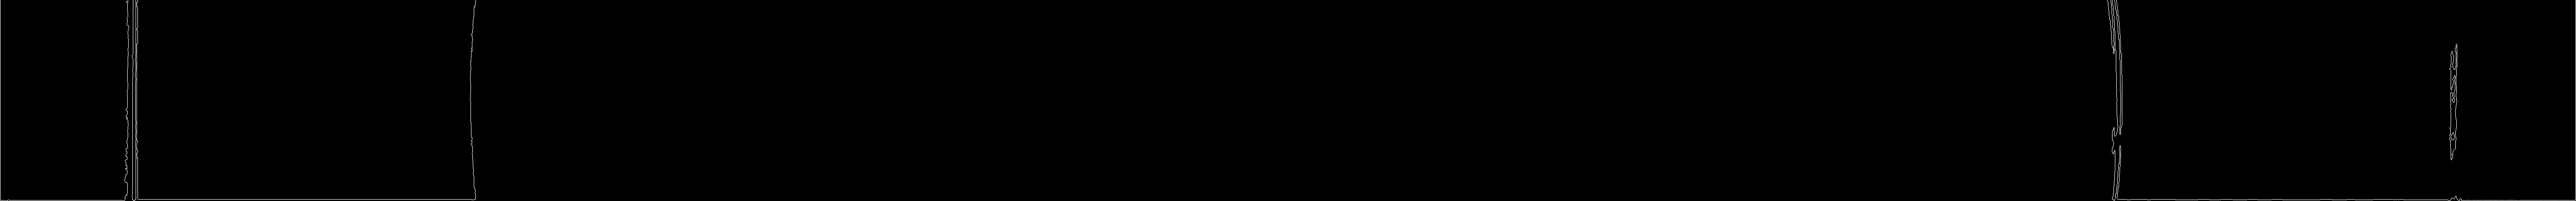
\includegraphics[width=0.8\textwidth]{images/only_con_cut.jpg} % second figure itself
    \caption{Extrahierte Kontouren des Bildes ohne Pre-Processing, zugeschnitten 
    auf den (vermutlich) überlappenden Bereich}
    \label{fig:cons_cut}
\end{figure}

Dieses Verfahren wird auf beide Bilder angewendet. Daraus resultieren dann zwei 
zugeschnittene Bilder aus denen Konturen extrahiert wurden. 
Würden diese beiden Bildteile vollständig überlappen könnte jetzt der ICP-Algorithmus
angewendet werden. Dieser würde dann die korrekte Transformation berechnen in dem er 
die Konturen aus dem oberen Bild, mit denen aus dem unteren Bild vergleicht und die 
Distanz zwischen den Punkten minimiert. 
Der Grad der Überlappung ist unbekannt und kann nicht im Vorhinein bestimmt werden.
Dadurch kann der ICP-Algorithmus nicht eingesetzt werden. 
Eine andere wichtige Annahme kann getroffen werden: Jeweils eine Kontur aus 
dem oberen und unteren Bild haben mindestens einen gemeinsamen Punkt.

\section{Differenzierung von Punkten}

Die Distanz zwischen zwei Punkten kann über den euklidischen Abstand gemessen werden.
\cite{Dokmanic.2015}. Sei A ein Punkt in einer Kontur aus dem oberen Bild und K eine 
Kontur aus dem unteren Bild.  
Um den Punkt aus K zu finden, der am nächsten an A liegt, muss A mit jedem Punkt aus 
K verglichen werden. Das Punktepaar mit dem kleinsten gefunden Euklidischen Abstand 
wird als 'Best Match' gespeichert. Wenn die Euklidische Distanz null beträgt, kann 
die Suche abgebrochen werden, da kein kleinerer Wert mehr gefunden werden kann.
Dieser Ansatz ist dem ICP-Algorithmus ähnlich. Die Differenz zwischen zwei Konturen 
K1 und K2 kann verglichen werden, indem für jeden Punkt A aus K1 der näheste Punkt aus 
K2 gefunden wird. In dem ICP-Algorithmus werden alle Distanzen von der 'Best Matches' 
aufsummiert und beschreiben den Unterschied der beiden Distanzen. Diese Summe kann dann 
minimiert werden. Dieser Ansatz funktioniert bei einem sich nur partiell
überlappenden Datensatz nicht. 
Statt die Summe zu bilden, wird jede beste Distanz zusammen mit ihren korrespondieren 
Punkten gespeichert. Um den Grad der Überlappung zu bestimmen, werden die Distanzen 
gezählt die gleich null sind. Dieser Wert in Relation zu der Länge von K1 gibt, 
in Prozent, an zu welchem Anteil sich die beiden Konturen überlappen.

\section{Transformation bestimmen}

Gesucht ist die Transformation welche die maximale Überlappung der beiden 
Konturen K1 und K2 bietet. Um diese Transformation zu berechnen, muss der 
Grad der Überlappung für jede mögliche Positionierung ermittelt werden. Jeder
Punkt aus K2 muss auf die Koordinaten eines beliebigen aber festen Punkts aus K1 
verschoben werden.
Die Transformation zwischen zwei Punkten A und B kann über die Vektorberechnung erfolgen:

\begin{equation*}
    T_{a,b} = \begin{pmatrix}a_x\\a_y\end{pmatrix} - \begin{pmatrix}b_x\\b_y\end{pmatrix}
\end{equation*}

Kontur K2 kann über Kontur K1 verschoben werden, indem Punkt A festgehalten wird, 
während Punkt B sukzessive jeden Punkt aus K2 annimmt. 
Die daraus resultierende Punkttransformation wird auf jeden Punkt von K1 angewendet, 
um die nächstgelegenen Nachbarpunkte zu ermitteln. Für jede Transformation wird der 
Überlappungsanteil berechnet, wobei das Ergebnis mit der maximalen Überlappung
als die optimale Transformation gespeichert wird.
Dieses Verfahren ist nur anwendbar, wenn Punkt A im überlappenden Bereich liegt. 
Befindet sich Punkt A nicht in der Kontur K2, 
kann das Verfahren nicht erfolgreich angewendet werden.
Zur Berechnung der optimalen Transformation werden verschiedene Punkte aus K1 
ausgewählt und das Verfahren jeweils angewendet. 
Die Transformation mit dem größten Verhältnis von Nullen zur
Gesamtlänge der Kontur wird als optimal angesehen. 
Aufgrund des exponentiellen Laufzeitverhaltens ist es ineffizient, 
jeden Punkt A aus K1 mit jedem Punkt B aus K2 zu vergleichen.

In Abbildung \ref{fig:before_matching} sind zwei Beispielkonturen zu sehen. 
Diese sind nicht angeordnet. Der ICP-Algorithmus würde diese beiden Konturen 
annähern, ohne sie zu überlappen. 
Das Ergebnis des vorgestellten Stitching Verfahrens ist in Abbildung 
\ref{fig:after_matching} zu sehen. Es ist zu erkennen das, trotz Messfehler und 
kleineren unterschieden im überlappenden Bereich die korrekte Transformation 
ermittelt werden konnte. Diese Konturen stammen von einem additiv gefertigten 
Metallbauteil.

\begin{figure}[h]
    \centering
    \begin{minipage}{0.49\textwidth}
        \centering
        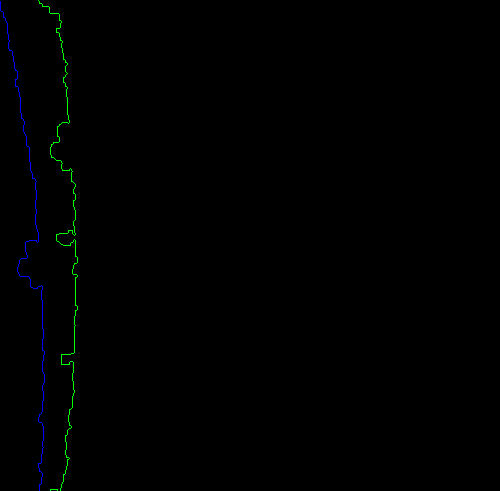
\includegraphics[width=\textwidth]{images/before_matching.png} % first figure itself
        \caption{Konturen, vor der Transformation}
        \label{fig:before_matching}
    \end{minipage}
    \begin{minipage}{0.49\textwidth}
        \centering
        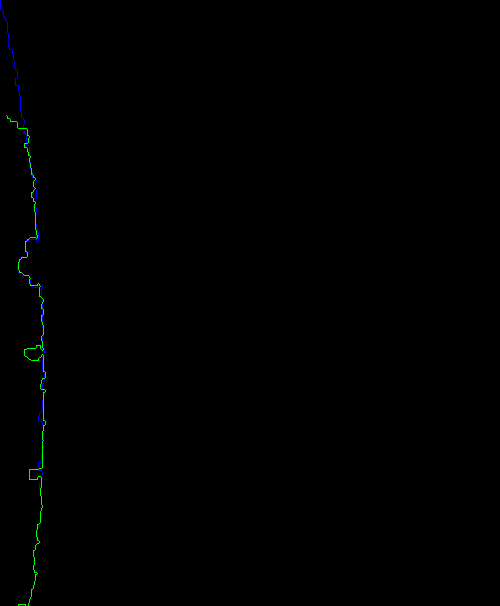
\includegraphics[width=\textwidth]{images/0.24225865209471767contours.png} % first figure itself
        \caption{Konturen, transformiert mit größter Überlappung, 
        Grad der Überlappung: 24,26\%}
        \label{fig:after_matching}
    \end{minipage}\hfill
\end{figure}

\section{Stitching visuell dargestellt}

Von Abbildung \ref{fig:stitching_beginn} bis \ref{fig:stitching_end}
ist der Prozess des Verfahrens zu sehen. K1 ist in Blau dargestellt, K2 in Grün.
In jeden Bild ist der Grad der Überlappung dargestellt. Es ist dargestellt wie
Kontur K2 über K1 geschoben wird, um den besten Grad der Übereinstimmung zu ermitteln.
Die Bilder sind repräsentativ ausgewählt, im tatsächlichen Prozess wird K1 komplett 
über K2 bewegt.

\begin{figure}[h]
    \centering
    \begin{minipage}{0.24\textwidth}
        \centering
        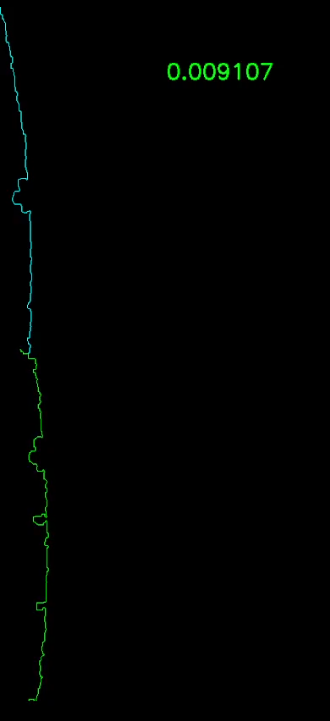
\includegraphics[width=\textwidth]{images/stitching_beginn.PNG} % first figure itself
        \caption{Konturen K1 und K2 beim Beginn des Verfahrens}
        \label{fig:stitching_beginn}
    \end{minipage}
    \begin{minipage}{0.24\textwidth}
        \centering
        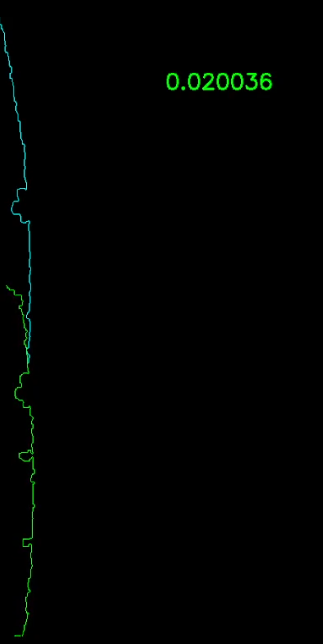
\includegraphics[width=\textwidth]{images/stitching_middle.PNG} % first figure itself
        \caption{Konturen K1 und K2 nach n Schritten}
        \label{fig:stitching_middle}
    \end{minipage}\hfill
    \begin{minipage}{0.24\textwidth}
        \centering
        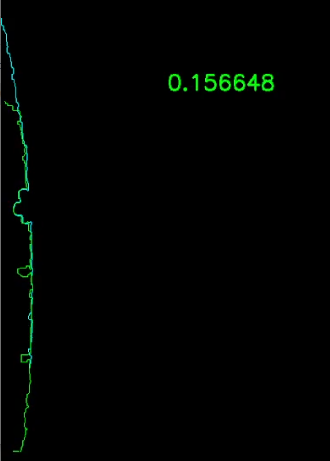
\includegraphics[width=\textwidth]{images/stitching_match.PNG} % first figure itself
        \caption{Konturen K1 und K2 beim einer guten Übereinstimmung}
        \label{fig:stitching_match}
    \end{minipage}\hfill
    \begin{minipage}{0.24\textwidth}
        \centering
        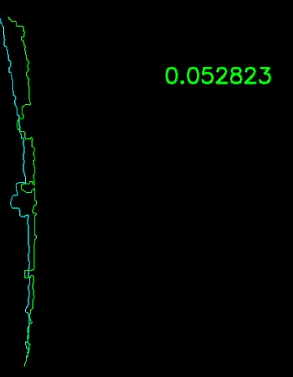
\includegraphics[width=\textwidth]{images/stitching_end.PNG} % first figure itself
        \caption{Konturen K1 und K2 beim Ende des Verfahrens}
        \label{fig:stitching_end}
    \end{minipage}\hfill
\end{figure}

\section{Bilder zusammenfügen}

Wenn alle Transformationen vorliegen wird die Transformation mit der besten 
Übereinstimmung gewählt. Diese wird genutzt, um die beiden Bilder zusammenzufügen.
Das zugehörige Bild der Konturen K2 wird transformiert, indem die Transformation 
auf jeden Pixel angewendet wird.  
Die Transformation ist nur korrekt, wenn die beiden Bilder die gleichen 
Ursprungskoordinaten haben, die auch bei den Konturen K1 und K2 verwendet wurden.

\begin{figure}[h]
    \centering
    \includegraphics[width=0.8\textwidth]{images/AM_SP0_stitched_2.png} % first figure itself
    \caption{Zusammengefügtes Bild}
    \label{fig:stitched_image}
\end{figure}

\section{Probleme und Lösungen im Verfahren}

Durch die Funktionsweise treten am Randbereich der Scannerdaten vermehrt Messfehler auf, 
die nicht vollständig durch vorheriges Filtern entfernt werden können. 
Damit diese Messfehler das Stitching nicht verfälschen, werden alle Konturen nochmals 
gefiltert. Alle Punkte in einer Kontur, die sich in einem konfigurierbaren 
Abstand zu den Bildrändern befinden, werden entfernt. Dadurch werden sie bei der 
Berechnung der Transformation nicht verwendet. 
Der konfigurierbare Abstand muss beim Stitching des finalen Bilds berücksichtigt 
werden und von der Transformation abgezogen werden.

Wenn Konturen mit einem großen Längenunterschied verglichen werden, 
kann eine sehr hohe Übereinstimmung ermittelt werden, die aber keine 
tatsächliche Übereinstimmung ist. Dies liegt daran, dass es wahrscheinlicher ist 
eine Sequenz der Länge 5 in einer anderen Sequenz der Länge 500 zu finden.  
Das kann zum Beispiel vorkommen, wenn Konturen 
die am linken und rechten Bildrand in Abbildung \ref{fig:cons} zu sehen sind, 
verglichen werden. Um dies zu vermeiden wird eine Bedienung eingeführt, dass die Länge
der Konturen nicht zu sehr voneinander abweichen darf. Bei einer Abweichung von mehr als
200 Punkten in einer Kontur sollte die Konturen nicht miteinander verglichen werden.

Auch Konturen mit einer Länge von weniger als 100 Punkten sollten nicht berücksichtigt 
werden. Diese beschreiben keine Features in einem Bild, die für das Stitching verwendet 
werden sollten. Diese Konturen beschreiben meist nur Messfehler oder 
Oberflächenstrukturen, die nicht konsistent in beiden Bildern von dem Scanner erkannt 
werden können.

Um das Ergebnis noch weiter zu verbessern, können zwei Konturen zweimal miteinander 
verglichen werden. Während des zweiten Vergleichs wird die Zielkontur mit der 
Ursprungskontur vertauscht. So wird aus beiden Konturen jeweils einmal ein fester 
Punkt gewählt. Wieder wird die Transformation gespeichert mit der besten Überlappung.
Wenn die Überlappung im zweiten Vergleich eine höhere Übereinstimmung hat, muss die 
berechnete Transformation invertiert werden. Geschieht dies nicht, kann die 
Transformation nicht für den finalen Stitchprozess eingesetzt werden, weil dort 
das Ziel und Ursprungsbild fest gesetzt ist.
